% !TEX root = illustrator_submission.tex

\section{Transparency Groups}
\label{sec:transparency-groups}

In Section~\ref{sec:blendmodes}'s discussion of blend modes, we assumed objects are simply blended in object stacking
order with blend modes directing the blending.
The PDF~1.4 transparency model becomes more intricate when graphics objects are grouped.
Transparency groups, or simply {\em groups}, allow a sequence of consecutive objects to be
collected together and composited
to produce a single color and opacity at each color sample.  Groups facilitate independent sub-scenes
to be composited together.  Artists also use groups to combine objects for artistic effects such
as darkening or lightening regions.  Groups can be nested within other groups to form a tree of groups.
When a group is reduced to a single color and opacity, the group itself has a blend mode and a per-group opacity 
used to composite the group with its backdrop.
Transparency groups are a distinct concept from other mechanisms to
group objects such as groups formed to manage hierarchical
transforms or inherited properties.

\subsection{Isolated versus Non-isolated Groups}
\label{sec:transparency-groups}

Groups can be either {\em non-isolated} (\Illustrator/'s default for a new group) or
{\em isolated}.\footnote{The SVG Compositing specification \cite{SVG-Compositing-Spec}
has the same concept but calls the property {\em enable-background} where
the value {\em accumulate} matches non-isolated and {\em new} matches isolated.}
This distinction is
which backdrop is used when compositing objects in the group.  With a non-isolated group, the backdrop is ``inherited''
from whatever has already been rendered prior in the object stacking order.  This allows
a group to interact with the prior objects ``beneath'' the group.  With an isolated group, the backdrop is
fully transparent so it has neither color, shape, nor opacity.
This is sometimes called rendering ``on glass'' because there is really
nothing for the group to interact with when the group itself is rendered.  The group's rendering is---as the name implies---isolated.

Both modes are useful in their proper context.  Non-isolated groups make sense when rendering a group expects to
interact with the artwork beneath it.  For example, a non-isolated group makes sense when
an artist wants to use a blend mode such as {\em ColorDodge}
or {\em ColorBurn} where painting with black or white respectively preserves the backdrop color.  Compositing
a source object using these blend modes with an isolated group would not make much sense because the 
initial backdrop is fully transparent so there is no color to preserve.

Isolated groups are more appropriate when the group is considered
a fully resolved piece of artwork you simply want to composite into the scene.  For example, a piece of
vector clip art consisting of objects rendered with the {\em Normal} blend mode and
that otherwise has no blending relationship with what's been rendered so far.

\subsubsection{Framebuffer Management for Groups}
\label{sec:isolated-groups}

Of the two types of groups, non-isolated is the more expensive to implement.  Both types of groups
conceptually create a transient framebuffer necessary to resolve the color, shape, and opacity of the group.
We call this a {\em framebuffer instance} and we implement the group's framebuffer instance with an OpenGL framebuffer object
(FBO) distinct
from the current framebuffer instance.  Allocating and discarding transient FBOs during rendering
is inefficient so we manage a set of framebuffer resources sufficient to handle the scene's maximum
non-trivial group nesting.  Each framebuffer instance needs independent color buffer storage---and CMYK needs multiple
color buffers as Section~\ref{sec:representing-cmyk} discusses.  However all the framebuffer instances can share
a single stencil buffer.  This stencil sharing is useful for maintaining the clip path nesting and conserving GPU
memory usage.  Because each FBO used to manage transient layers is preallocated and may be used to render a
group positioned
arbitrarily 
within the scene's viewport, each FBO is maintained at the same dimensions as the base framebuffer instance (typically sized to match the maximum window-space view size) and expects to share a single stencil buffer.

We speak of {\em non-trivial} groups because in common cases where every blend mode within a group is {\em Normal}
and the group opacity is fully opaque (and other uncommon group features such as knock-out are inactive),
rendering a group to its own framebuffer instance is functionally identical
to simply rendering the group's objects in sequence into the current framebuffer instance. Recognizing trivial
groups and not instantiating a framebuffer instance for them is an important performance optimization.

But in cases when a non-trivial group is present, we carefully orchestrate rendering to a framebuffer
instance and when the group is resolved, compositing the resolved framebuffer layer for the group back into
the previously current framebuffer layer.  Because groups can be nested to form a tree, this process is
conceptually recursive but practically limited by the scene's maximum non-trivial group nesting.

From this point on, our discussion deals with non-trivial groups.

\subsubsection{Implementing Non-isolated Groups}
\label{sec:non-isolated-groups}

\begin{figure}[tb]
  \center{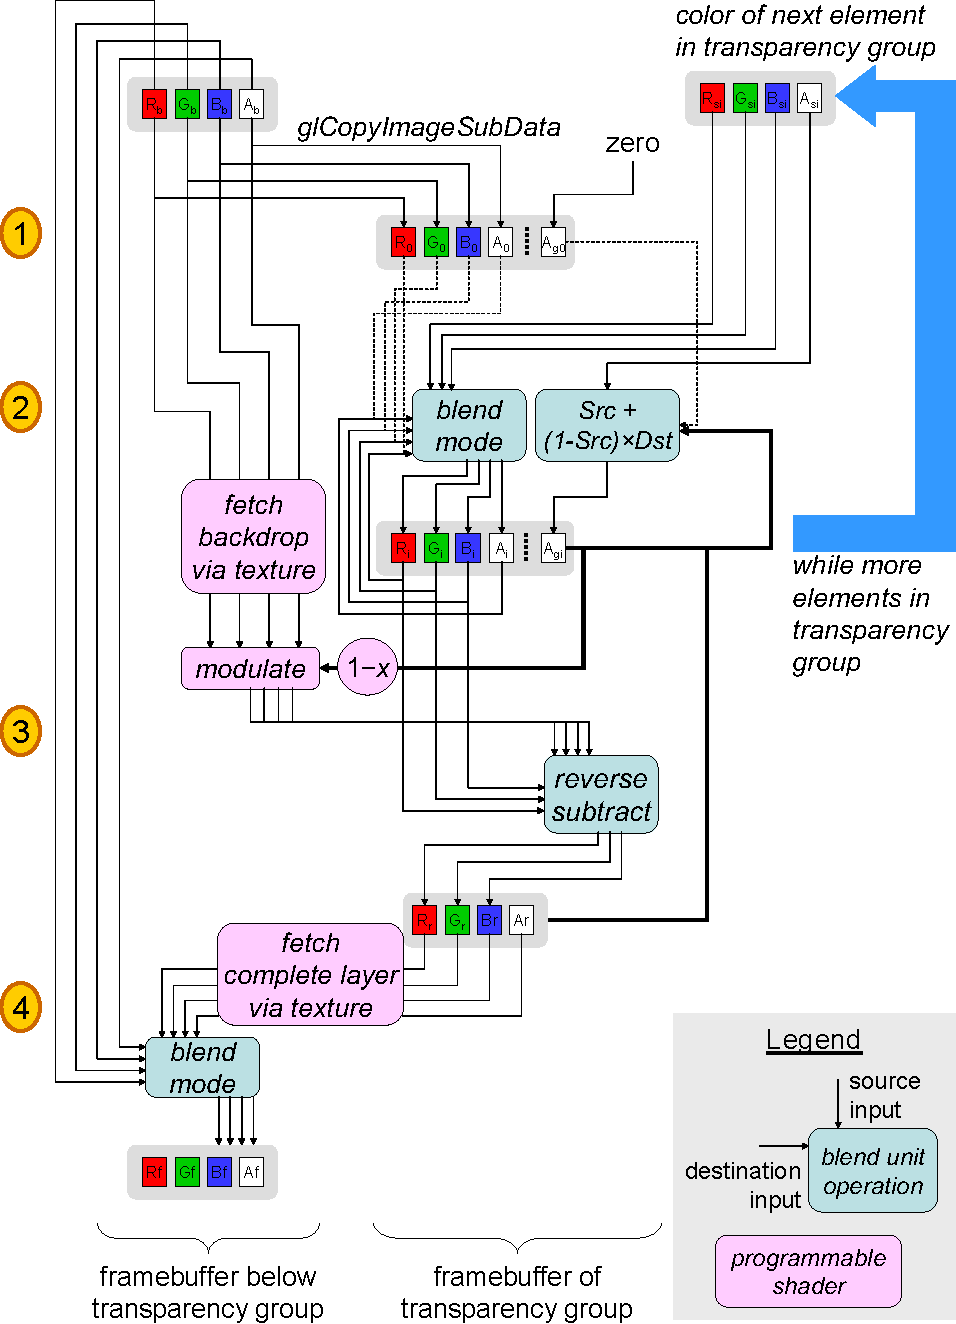
\includegraphics[width=\columnwidth]{images/non_isolated_group.pdf}}
  \caption{\label{fig:non-isolated-group} Four steps in rendering a non-isolated group with the GPU.}
\end{figure}

Figure~\ref{fig:non-isolated-group} illustrates the steps to process and resolve a non-isolated group
assuming an RGB color space.
Numbered circles down the figure's left side indicate the steps 1, 2, 3, and 4 to be discussed in turn.

{\bf Step 1:}
Establishing a non-isolated group requires copying the backdrop from the current framebuffer instance
to the group's transient FBO's color buffer(s).  OpenGL's {\tt glCopyImageSubData} command \cite{CopyImageSpec} copies
a rectangular region of texel color values
from one color buffer's underlying texture object to another.  When the color buffers are multisampled, the command
copies each pixel's individual color samples.  In the worst case, we may have to copy the entire
color buffer contents but often we can bound the window-space bounding box for the objects within the
group (including any nested groups).  CMYK has multiple color buffers configured as layers of
a texture array but a single {\tt glCopyImageSubData} command can copy all the texture array layers.

An additional single-component (red) color buffer is also required for the FBO to maintain the non-isolated group's
{\em group alpha} and labeled $A_{g0}$  and $A_{gi}$ in the Figure~\ref{fig:non-isolated-group}.
A scissored {\tt glClear} command must clear the {\em group alpha} color buffer to zero
The motivation for {\em group alpha} will be more clear in Step~3.

{\bf Step 2:}
Each element of the group must be rendered in object stacking order.  Any object that is a non-trivial
group requires that nested group to be rendered and resolved.  In such cases, the resolved color and opacity
of the nested group is composited using the group element's blend mode and group opacity into this
framebuffer instance.  Elements of trivial groups can simply be rendered in sequence.

During step 2, in addition to compositing group elements into the RGB color buffer (or buffers for CMYK),
the {\em group opacity} buffer is configured for PDF's {\em Normal} blending (implemented in OpenGL with
the {\tt GL\_ONE,GL\_ONE\_MINUS\_\-SRC\_ALPHA} blend function).  The fragment shader is responsible to output
the alpha of each group element to this color buffer.  The {\em group alpha} buffer is used to keep
a distinct running accumulation of alpha but starting from zero from the alpha component(s) in the
other (4-component) color buffers.

{\bf Step 3:} 
Before the resolved color in a non-isolated group can be composited back to the prior
framebuffer instance from before processing the group, we must ``subtract out'' the backdrop color and alpha
used to initialize the group's framebuffer instance by {\tt glCopyImageSubData}.  Otherwise when the
resolved color of the group is composited back into the prior framebuffer instance (Step~4), the
prior framebuffer instance's color and alpha would be accounted for twice.

The PDF specification computes the resolved result of a non-isolated transparency group with the equations:
\begin{align}
\label{eq:straight-non-isolated-color}
C & = C_n + (C_{n} - C_{0}) \times \left( \frac{\alpha_{0}}{\alpha_{gn}} - \alpha_{0} \right) \\
%
\label{eq:straight-non-isolated-alpha}
\alpha & = \alpha_{gn}
\end{align}
where $C$ is the resolved group color, $C_{n}$ is the final color in the framebuffer instance after all $n$ group
elements are composited, $C_{0}$ and $\alpha_{0}$ are the backdrop color and alpha respectively
from the prior framebuffer instance, and $\alpha_{gn}$ is the final {\em group alpha} from the
single-channel color buffer after all $n$ group elements are composited.

This equation is written with non-premultiplied alpha but the GPU represents colors in pre-multiplied alpha form.
Combining the Equations~\ref{eq:straight-non-isolated-color} and \ref{eq:straight-non-isolated-alpha} to find $\alpha C$ simplifies to:
\begin{equation}
\label{eq:premult-non-isolated}
\alpha C = \alpha_{n} C_{n} \left( \frac{\alpha_{gn} + (1-\alpha_{gn}) \alpha_{0}}{\alpha_{n}} \right) - (1-\alpha_{gn}) \alpha_{0} C_{0}
\end{equation}
We recognize the fractional expression in Equation~\ref{eq:premult-non-isolated} reduces to unity
because  $\alpha_{gn} + (1-\alpha_{gn}) \alpha_{0}$ is $\alpha_{n}$ because 
the alpha composition of the final {\em group alpha} with the backdrop alpha $\alpha_{0}$ is simply $\alpha_{n}$
as alpha compositing is associative.

So Equation~\ref{eq:premult-non-isolated} simplifies to:
\begin{equation}
\label{eq:simple-premult-non-isolated}
\alpha C = \alpha_{n} C_{n} - (1-\alpha_{gn}) \alpha_{0} C_{0}
\end{equation}
Equation~\ref{eq:simple-premult-non-isolated} can be realized in OpenGL by rendering a conservative window-space rectangle
matching the rectangle used for the earlier {\tt glCopyImageSubData} command with this subtractive blend
\begin{verbatim}
  glBlendEquation(GL_FUNC_REVERSE_SUBTRACT);
  glBlendFunc(GL_ONE, GL_ONE);
\end{verbatim}
and a per-color sample fragment shader that outputs the product of fetching color values from the prior framebuffer
instance to get $C_{0}$ and one minus the texel $\alpha_{gn}$ fetched from the single-component {\em group
alpha} color buffer.

{\bf Step 4:} 
Lastly composite the resolved group color $\alpha C$ and opacity $\alpha$ back to the prior framebuffer instance by
rendering
with per-sample shading
another conservative window-space rectangle, here applying the blend mode for the group.
The logical Steps 3 and 4
can be advantageously combined into a single rendering pass.

\subsubsection{Implementing Isolated Groups}
\label{sec:isolated-groups}

Isolated groups are easier.
The isolated group rendering process follows the same general structure as shown in
Figure~\ref{fig:non-isolated-group} except Step 1 simply clears the group's framebuffer instance color buffer(s)
to fully transparent.  For RGB, this is clearing the color buffer to zero.  For CMYK, this is clearing the
RGB components to one and alpha component to zero.  No {\tt glCopyImageSubData} command is necessary.

Since an isolated group does not copy the backdrop from the prior framebuffer instance,
there is also no need to ``subtract out'' that backdrop in Step 3 so this step can be skipped.

Steps~2 and 4 operate in the same manner as for non-isolated groups.

\subsection{Knockout}
\label{sec:knockout}

By default, groups composite the elements of the group in their stacking
order and use the prior element's rendering result as their backdrop.
A group marked for knockout, known as a {\em knockout group}, always
uses the group's initial backdrop.  One common use of knock-out is
rendering semi-opaque annotations where the annotations may overlap but
double-blending of annotations is undesirable so only the last rendered annotation at
any given pixel should blend with the prior framebuffer instance (the
backdrop).

``Stencil, then cover'' path rendering provides an efficient way to
implement knockout by rendering the elements of the group in reverse
stacking order.  Blend normally during the ``cover'' step but mark every
updated stencil sample by setting an upper bit in the stencil buffer
for each updated color sample.  Then have further rendering by other
elements in the knockout group fail the stencil test if the stencil sample
value's upper bit is set.  This ensures color samples are only updated
and blended by the last element in the group's stacking order to cover
the color sample.  When all the group's elements have been rendered,
draw a conservative covering rectangle to unmark the stencil values so
normal ``stencil, then cover'' rendering can proceed.

Note that this
%{\em Caveat:} This
approach will not work if any of the immediate
elements of the knockout group are non-isolated-groups.
This uncommon case requires the non-isolated group element to use the
backdrop of prior group elements in the stacking order which the reverse
order will not have rendered so an explicit and involved knockout approach
is required.

% TOO LONG
%\subsection{Additional Transparency Features}
%
%Additional features of the PDF transparency model (soft masks, {\em
%alpha-is-shape}, page groups, and overprint) must also be GPU-accelerated
%and are mentioned here for completeness but are beyond the scope of this
%presentation due to space constraints and their relative unimportance
%compared to the other features discussed here.

